%%%%%%%%%%%%%%%%%%%%%%%%%%%%%%%%%%%%%%%%%%%%%%%%%%%%%%%%%%%%%%%%%%%%%%%
%% Optionen zum Layout des Artikels                                  %%
%%%%%%%%%%%%%%%%%%%%%%%%%%%%%%%%%%%%%%%%%%%%%%%%%%%%%%%%%%%%%%%%%%%%%%%
\documentclass[%
  %a5paper,
]
{scrartcl}

%\pagestyle{empty}		% keine Kopf und le (k. Seitenzahl)
%\pagestyle{headings}	% lebender Kolumnentitel


%% Deutsche Anpassungen %%%%%%%%%%%%%%%%%%%%%%%%%%%%%%%%%%%%%
\usepackage[ngerman]{babel}
\usepackage[T1]{fontenc}
\usepackage[utf8]{inputenc}
\usepackage{amsmath}
\usepackage{amsfonts}
\usepackage{amssymb}
\usepackage{lmodern} %Type1-Schriftart
%Für das verlinkte Inhaltsverzeichnis
\usepackage[colorlinks,pdfpagelabels,pdfstartview = FitH,bookmarksopen = true,bookmarksnumbered = true,linkcolor = black,plainpages = false,hypertexnames = false,citecolor = black] {hyperref}
\usepackage{wrapfig}

%
\usepackage{graphicx} %%Zum Laden von Grafiken
\usepackage{subfig} %%Teilabbildungen in einer Abbildung
%\usepackage{tikz} %%Vektorgrafiken aus LaTeX heraus erstellen

\relpenalty=9999	%verhindert Trennung von $...$
\binoppenalty=9999


%% Bibliographiestil %%%%%%%%%%%%%%%%%%%%%%%%%%%%%%%%%%%%%%%%%%%%%%%%%%
%\usepackage{natbib}

\begin{document}



%%%%%%%%%%%%%%%%%%%%%%%%%%%%%%%%%%%%%%%%%%%%%%%%%%%%%%%%%%%%%%%%%%%%%%%
%% Ihr Artikel                                                       %%
%%%%%%%%%%%%%%%%%%%%%%%%%%%%%%%%%%%%%%%%%%%%%%%%%%%%%%%%%%%%%%%%%%%%%%%

%% eigene Titelseitengestaltung %%%%%%%%%%%%%%%%%%%%%%%%%%%%%%%%%%%%%%%
%\begin{titlepage}

%\end{titlepage}

%% Angaben zur Standardformatierung des Titels %%%%%%%%%%%%%%%%%%%%%%%%
%\titlehead{Titelkopf }
%\subject{Typisierung}
\title{Das Ising-Modell mit Monte-Carlo und Metropolis}
\author{Christian Darsow-Fromm
\and{Maximilian Menzel}}
%\publishers{Herausgeber}

%% Widmungsseite %%%%%%%%%%%%%%%%%%%%%%%%%%%%%%%%%%%%%%%%%%%%%%%%%%%%%%
%\dedication{Widmung}

\maketitle 						% Titelei wird erzeugt

%% Zusammenfassung nach Titel, vor Inhaltsverzeichnis %%%%%%%%%%%%%%%%%


%% Erzeugung von Verzeichnissen %%%%%%%%%%%%%%%%%%%%%%%%%%%%%%%%%%%%%%%
\tableofcontents			% Inhaltsverzeichnis
%\listoftables				% Tabellenverzeichnis
%\listoffigures				% Abbildungsverzeichnis

\setlength{\tabcolsep}{10pt}
\renewcommand{\arraystretch}{2}

%% Der Text %%%%%%%%%%%%%%%%%%%%%%%%%%%%%%%%%%%%%%%%%%%%%%%%%%%%%%%%%%%

\section{Das Ising-Modell}
Das Ising-Modell ist eine Vereinfachung des Heisenberg-Modells. Die Spins werden nicht als Vektor behandelt, sondern auf $s_i^z = \pm 1$ reduziert.
\begin{equation}
  \hat{\mathcal H} = -\frac 12\sum _{ij} J_{ij} S_i^z S_j^z - B_z \sum_{i=1}^N S_i^z  \label{eq:IsingHamilton}
\end{equation}
%TODO schöne Einleitung
Deshalb ist das Ising-Modell vor allem dann eine gute Näherung des Heisenberg-Modells, wenn sich durch Anisotropien eine vorgezogene Richtung ergibt, oder wenn sich die Spins an einem Isotropen äußeren Magnetfeld ausrichten.
Um das Modell weiter zu vereinfachen, wird in der Regel für $J_{ij}$ eine nächste-Nachbar-Wechselwirkung angenommen. $J$ ist konstant für das gesamte System und es wird nur die Wechselwirkung mit den direkten Nachbarn berechnet.

Mit dem Modell kann der Phasenübergang eines Ferromagneten in zwei und mehr Dimensionen beschrieben werden.
\section{Die Monte-Carlo Methode}

\section{Die Implementierung}

\subsection{Die Architektur}
\begin{wrapfigure}{r}{8.5cm}
  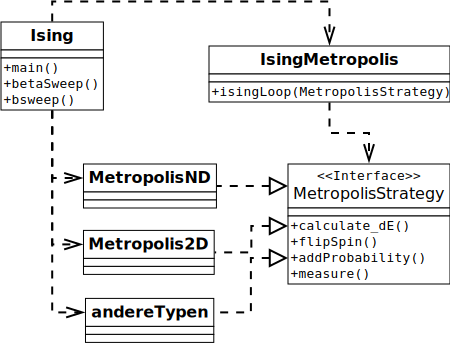
\includegraphics[width=0.6\textwidth]{bilder/impl/strategy.png}
  \caption{Darstellung des Strategie-Patterns \label{strategyPattern}}
\end{wrapfigure}
Unser Code ist lässt sich ein primär 3 Bestandteile zerlegen: \textit{Ising.cpp} dient als Einstiegspunkt, \textit{IsingMetropolis.cpp} definiert den Algorithmus und \textit{MetropolisStrategy.h} beschreibt die Struktur der Probe.

Die drei Teile sind durch das Strategie-Pattern, wie in Abbildung \ref{strategyPattern} dargestellt, lose gekoppelt. 
Beim Strategie-Pattern wird ein (abstrakter) Algorithmus definiert und die Strategie als Parameter übergeben. Im Algorithmus werden dann Methoden der Strategie ausgeführt. 

Der Vorteil dieses Designpatterns liegt darin, dass die Strategie, in unserem Fall die Struktur der Probe, austauschbar ist, ohne die Implementierung des Algorithmus' zu verändern; es muss lediglich eine neue Klasse das Strategie-Interface implementieren.

\subsection{Simulationsstart}
In \textit{Ising.cpp} werden die Parameter eingelesen. Sie können entweder über die Konsole oder über eine Konfigurationsdatei angegeben werden. Je nach Angabe der Parameter kann entschieden werden was für eine Simulation (B-Feld-Sweep, Temperatur-Sweep) mit welcher Strategie gestartet werden soll. Zudem werden die Ausgaben der Simulation gesteuert.

Beim Temperatur-Sweep wird $\beta = \frac{1}{k_B T}$ (wobei $k_B = 1$) im angegebenen Intervall in äquidistanten Schritten variiert. Da jede Temperatursimulation von den anderen unabhängig ist konnte diese Messreihe leicht mit \textit{OpenMP} parallelisiert werden. Dazu wird für jeden Thread eine Kopie der Strategie erstellt (\textit{clone()}) und die for-Schleife mit \textit{\#pragma omp for} parallelisiert. Es werden für jede Temperatur ein Bild mit der letzten Spin-Konfiguration und eines mit den Mittelwerten ausgegeben. Die Messewerte ($\beta$, mittlere Magnetisierung pro Spin und mittlere Fliprate) werden in der Konsole ausgegeben.

Mit B-Feld-Sweep lässt sich eine Hysterese-Kurve aufzeichnen. Dazu wird mit der selben Strategie B-Felder (in äquidistanten Schritten) durchlaufen: \begin{equation} 0 \to B_{max} \to B_{min} \to B_{max} \nonumber \end{equation}
Da nun aber jeder Schritt (im B-Feld) der Simulation auf dem vorherigen aufbaut, ließ sich dies nicht mit \textit{OpenMP}  parallelisieren. 
Es werden ebenfalls Bilder für jeden Schritt ausgegeben und die Messwerte ($B$, mittlere Magnetisierung pro Spin und mittlere Fliprate) in die Konsole geschrieben.

\subsection{Implementation des Algorithmus'}
Weil das Strategie-Pattern verwendet wird, definiert \textit{IsingMetropolis.cpp} nur die Struktur, die bereits in Abschnitt \ref{sec:MonteCarloMethode} beschrieben ist. Die Berechnung der Energiedifferenz, das Flippen der Spins, die Wahrscheinlichkeitszählung und die Messung sind ausgelagert.  Nur das Bestimmen des zufälligen Spins und die Flipwahrscheinlichkeit
(nach \eqref{eq:FlipChance}) sind nicht ausgelagert. Des weiteren wird die Anzahl der Flips mit gezählt, um die Aktivität des Systems erfassen zu können. 


\subsection{Die Metropolis-Strategie}
Die Schnittstelle der Strategie ist in  \textit{MetropolisStrategy.h} beschrieben. Für den Metropolis-Algorithmus wichtigen Funktionen sind:
\begin{list}{}{}
\item  \textit{spinNumber()} zur Bestimmung der Spinanzahl (Maximum für Zufallsspin)
\item  \textit{calculate\_dE(int i)} Bestimmt die Energiedifferenz, wenn Spin \textit{i} flippte
\item  \textit{flipSpin(int i)} Flippt den Spin \textit{i}
\item  \textit{addProbability(int i)} Zeichnet den Wert des Spins \textit{i} auf (nach \eqref{eq:RekursiverMittelwert})
\item  \textit{measure()} Vermisst das System über den Erwartungswert (nach \eqref{eq:MagErwartungswert})
\end{list}
Die restlichen Methoden dienen zur Simulationssteuerung (\textit{reset()} , 
\textit{resetMeasure()} , 
\textit{setBField(double)} , 
\textit{clone()})  bzw. zur Bildausgabe. 

Wir verwenden nur eine Strategie, da sie die anderen darstellen kann und andere (noch) nicht implementiert sind: \textit{MetropolisND}. Es ist aber denkbar, dass z.B. eine Strategie mit Störstellen, eine anderer Gitteraufteilung (z.B. eine hexagonale Struktur) oder nicht nur nächste-Nachbarn-Näherung hinzugefügt werden.

\paragraph{MetropolisND}
Sowohl der Zugriff von außen (um die Schnittstelle allgemein zu halten) als auch die Speicherung der Spins (siehe Abschnitt \ref{sec:SpinArray}) erfolgt in linearer Weise. Da aber die nächste-Nachbar-Wechselwirkung in alle Dimensionen verläuft, ist eine Transformation des linearen Index' in eine ND-Koordinate notwendig. Zur Transformation wird einen Abwandlung des ''Turning-Weels''-Algorithmus' (wird verwendet um ein Kartesisches Produkt zu bilden, unser Algorithmus nummeriert quasi diese Elemente) verwendet. Der Index berechnet sich durch
\begin{equation}
i = \sum_{j=1}^D{ c(j)  \prod_{d=1}^{j-1} { s(d) }}
\end{equation}
wobei $D$ die Anzahl der Dimensionen angibt, $c(j)$ der Wert der Koordinate $j$ und $s(d)$ die Größe in der Dimension $d$ ist. 
Zum Berechnen der Koordinate wird die Ganzzahldivision und der Modulo verwendet:
\begin{equation}
c(j) = \frac{i}{\prod_{d=1}^{j-1} {s(d)} } \mod s(j) 
\end{equation}

Die Berechnung der Energiedifferenz nach Gleichung \eqref{eq:EnergieDiff} ist aufwendig, da sowohl die Gesamtenergie des Systems $S$ als auch $S'$ berechnet werden muss. Betrachtet man nun den Hamiltonoperator \eqref{eq:IsingHamilton}, läge die Laufzeit der Berechnung in $\mathcal O(N^2)$, wobei $N$ die Anzahl  der Spins ist; betrachtet man nur noch die nächste-Nachbar-Wechselwirkung, ist diese nur noch in $\mathcal O(N\cdot z)$, wobei $z$ die Anzahl der nächsten Nachbarn ist.
Da sich zum einen nur eine Spin verändert, nur die nächsten Nachbarn betrachtet werden, $J_{ij} = J$ konstant für das ganze System ist und nicht die Einzelenergien sondern die Energiedifferenz benötigt werden, vereinfacht die Berechnung der Energiedifferenz: 
\begin{align}
\Delta    E &= J \Delta S_i \sum_{j=n.n.} S_j + B \Delta S_i \\
\Delta S_i &= S_i - S'_i = \pm 2
\end{align}
Die Laufzeit ist nun in $\mathcal O(z)$ und hängt somit nicht mehr von der Größe des Systems ab (sofern man nicht die Anzahl der Dimensionen erhöht). Daher ist ein Berechnungsschritt für ein großes System genauso teuer wie das eines Kleinen.



\subsection{Spin-Array}
\label{sec:SpinArray}
Hierbei handelt es sich um eine effiziente Datenstruktur, die es erlaubt die Spin"=Konfiguration mit wenig Speicherbedarf zu verwalten.

Da jeder Spin im Ising-Modell nur 2 Werte annehmen kann, ist es möglich einen Spin mit einem einem Bit zu codieren. Daher besteht die Datenstruktur aus einem Bytearray, dessen Bits die Spins halten.

Es werden 3 einfache Methoden definiert: Zum Auslesen, Setzen und Flippen eines Spins. Alle drei Methoden sind ähnlich aufgebaut: Zuerst wird das Byte und dann das Bit dieses Bytes bestimmt, das den gewünschten Spin enthält, dann wir eine Bitoperation (and, or, xor) auf dieses Bit angewendet und entweder das neue Byte im Array gespeichert oder den Wert des Spins zurückgegeben.


\include{simulation}

%\bibliography{literatur}
%\bibliographystyle{alpha}
\end{document}
